% ============================================================================
% Figure include for the untied hyper-encoder section.
% Usage:  % ============================================================================
% Figure include for the untied hyper-encoder section.
% Usage:  % ============================================================================
% Figure include for the untied hyper-encoder section.
% Usage:  % ============================================================================
% Figure include for the untied hyper-encoder section.
% Usage:  \input{figure_untied}   (or copy this block into the section)
% Needs:  \usepackage{graphicx}   and  paper_fig_untied.pdf  on the graphics path.
% Two-column paper -> figure* (spans both columns, as below).
% Single-column paper -> replace figure*/figure and use width=\linewidth.
% ============================================================================

\begin{figure*}[t]
  \centering
  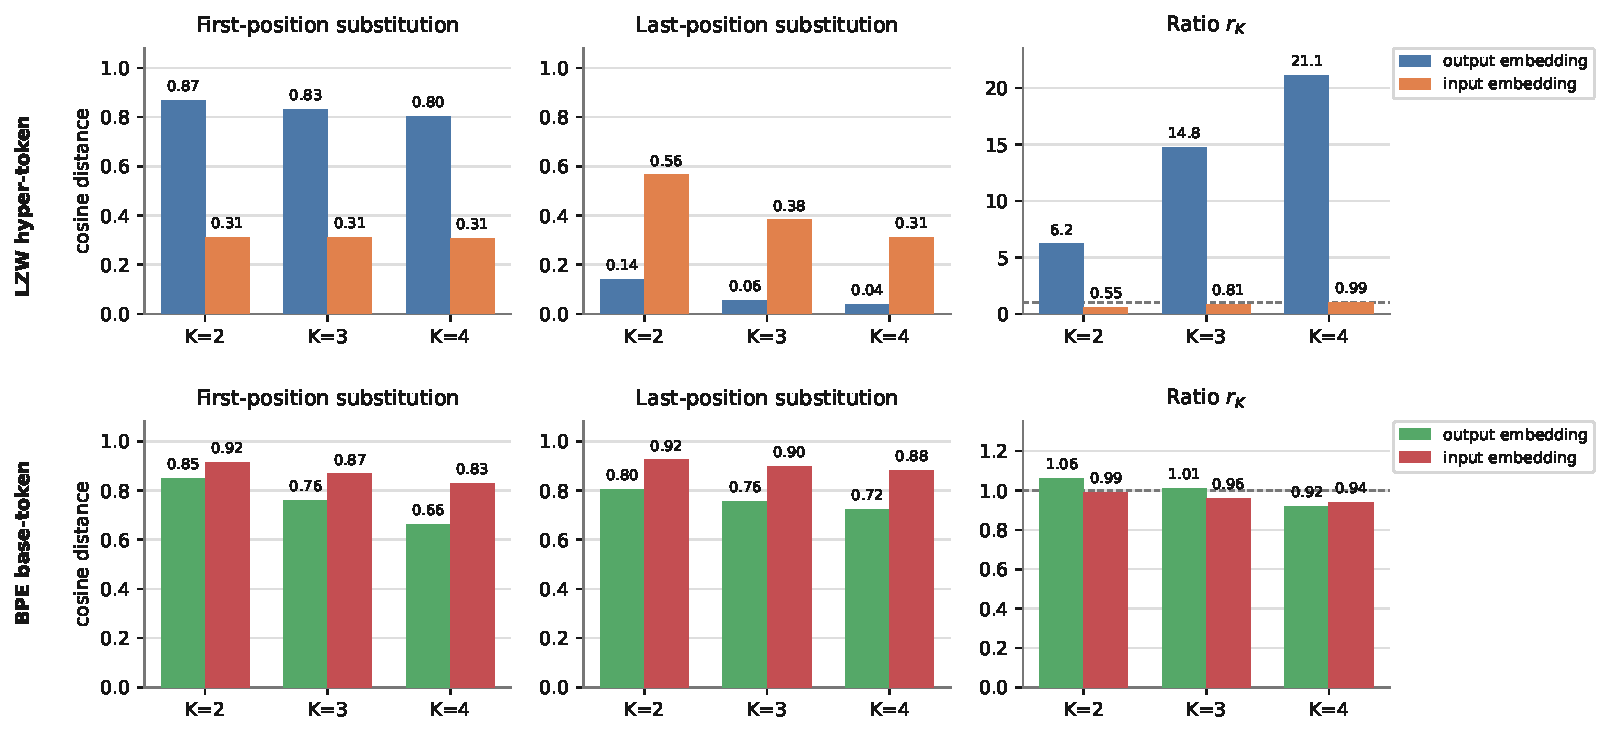
\includegraphics[width=0.92\textwidth]{paper_fig_untied.pdf}
  \caption{\textbf{The untied hyper-encoders learn complementary composition
  rules} (v0.6.4, WikiText-2). Colour encodes the role (blue = output, orange =
  input); line style encodes the model (solid = hyper-encoder, dashed = raw
  base-table control). \textbf{(a) Causal minimal pairs:} the ratio $r_K$ (log
  scale) of movement after replacing the first vs.\ the last constituent. The
  output hyper-encoder is strongly prefix-dominated and sharpens with span length
  ($r_4{=}20.9$), whereas the input hyper-encoder and \emph{both} base tables stay
  balanced ($r_K{\approx}1$). \textbf{(b) Nested-prefix similarity:}
  $\cos(H_2,H_K)$ as the span grows. The output representation stays high and
  decays slowly---its extensions share a prefix, so appending tokens barely moves
  it---while the input representation is lower and decays faster, tracking the
  span's changing meaning; the base control is low throughout, with no prefix
  effect.}
  \label{fig:untied-hyperencoders}
\end{figure*}
   (or copy this block into the section)
% Needs:  \usepackage{graphicx}   and  paper_fig_untied.pdf  on the graphics path.
% Two-column paper -> figure* (spans both columns, as below).
% Single-column paper -> replace figure*/figure and use width=\linewidth.
% ============================================================================

\begin{figure*}[t]
  \centering
  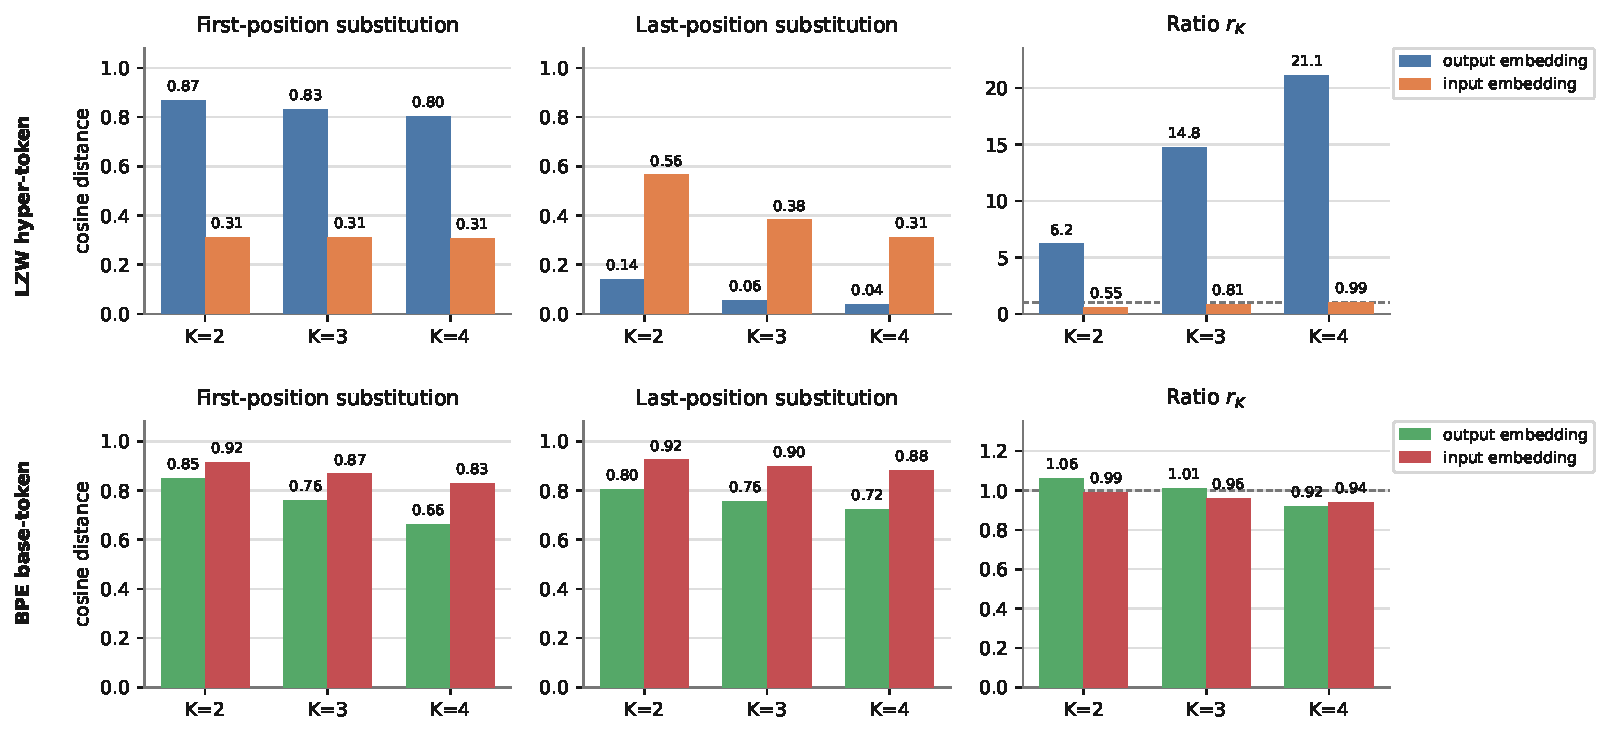
\includegraphics[width=0.92\textwidth]{paper_fig_untied.pdf}
  \caption{\textbf{The untied hyper-encoders learn complementary composition
  rules} (v0.6.4, WikiText-2). Colour encodes the role (blue = output, orange =
  input); line style encodes the model (solid = hyper-encoder, dashed = raw
  base-table control). \textbf{(a) Causal minimal pairs:} the ratio $r_K$ (log
  scale) of movement after replacing the first vs.\ the last constituent. The
  output hyper-encoder is strongly prefix-dominated and sharpens with span length
  ($r_4{=}20.9$), whereas the input hyper-encoder and \emph{both} base tables stay
  balanced ($r_K{\approx}1$). \textbf{(b) Nested-prefix similarity:}
  $\cos(H_2,H_K)$ as the span grows. The output representation stays high and
  decays slowly---its extensions share a prefix, so appending tokens barely moves
  it---while the input representation is lower and decays faster, tracking the
  span's changing meaning; the base control is low throughout, with no prefix
  effect.}
  \label{fig:untied-hyperencoders}
\end{figure*}
   (or copy this block into the section)
% Needs:  \usepackage{graphicx}   and  paper_fig_untied.pdf  on the graphics path.
% Two-column paper -> figure* (spans both columns, as below).
% Single-column paper -> replace figure*/figure and use width=\linewidth.
% ============================================================================

\begin{figure*}[t]
  \centering
  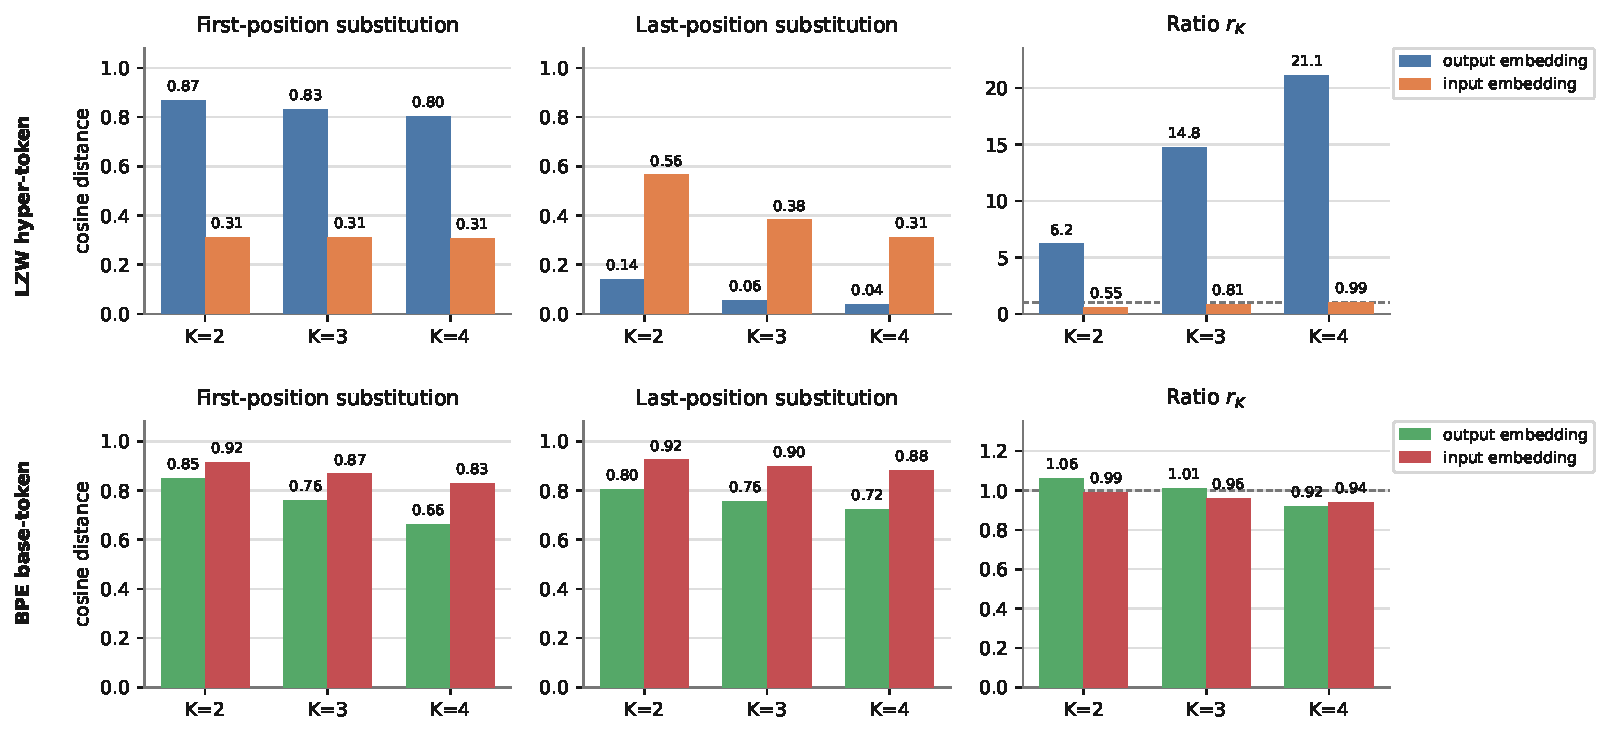
\includegraphics[width=0.92\textwidth]{paper_fig_untied.pdf}
  \caption{\textbf{The untied hyper-encoders learn complementary composition
  rules} (v0.6.4, WikiText-2). Colour encodes the role (blue = output, orange =
  input); line style encodes the model (solid = hyper-encoder, dashed = raw
  base-table control). \textbf{(a) Causal minimal pairs:} the ratio $r_K$ (log
  scale) of movement after replacing the first vs.\ the last constituent. The
  output hyper-encoder is strongly prefix-dominated and sharpens with span length
  ($r_4{=}20.9$), whereas the input hyper-encoder and \emph{both} base tables stay
  balanced ($r_K{\approx}1$). \textbf{(b) Nested-prefix similarity:}
  $\cos(H_2,H_K)$ as the span grows. The output representation stays high and
  decays slowly---its extensions share a prefix, so appending tokens barely moves
  it---while the input representation is lower and decays faster, tracking the
  span's changing meaning; the base control is low throughout, with no prefix
  effect.}
  \label{fig:untied-hyperencoders}
\end{figure*}
   (or copy this block into the section)
% Needs:  \usepackage{graphicx}   and  paper_fig_untied.pdf  on the graphics path.
% Two-column paper -> figure* (spans both columns, as below).
% Single-column paper -> replace figure*/figure and use width=\linewidth.
% ============================================================================

\begin{figure*}[t]
  \centering
  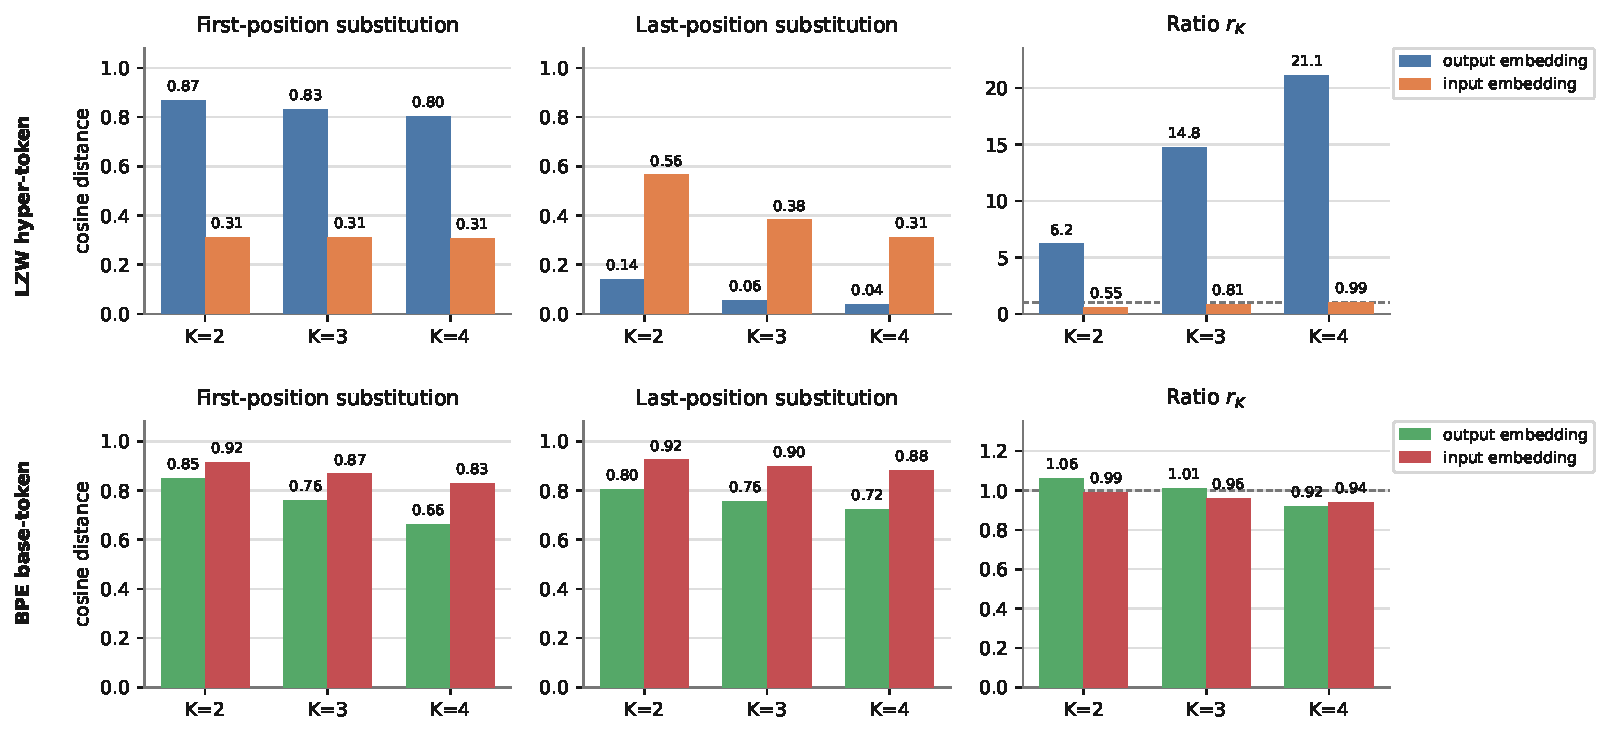
\includegraphics[width=0.92\textwidth]{paper_fig_untied.pdf}
  \caption{\textbf{The untied hyper-encoders learn complementary composition
  rules} (v0.6.4, WikiText-2). Colour encodes the role (blue = output, orange =
  input); line style encodes the model (solid = hyper-encoder, dashed = raw
  base-table control). \textbf{(a) Causal minimal pairs:} the ratio $r_K$ (log
  scale) of movement after replacing the first vs.\ the last constituent. The
  output hyper-encoder is strongly prefix-dominated and sharpens with span length
  ($r_4{=}20.9$), whereas the input hyper-encoder and \emph{both} base tables stay
  balanced ($r_K{\approx}1$). \textbf{(b) Nested-prefix similarity:}
  $\cos(H_2,H_K)$ as the span grows. The output representation stays high and
  decays slowly---its extensions share a prefix, so appending tokens barely moves
  it---while the input representation is lower and decays faster, tracking the
  span's changing meaning; the base control is low throughout, with no prefix
  effect.}
  \label{fig:untied-hyperencoders}
\end{figure*}
